\def\pescados{3}
\def\scal{5}
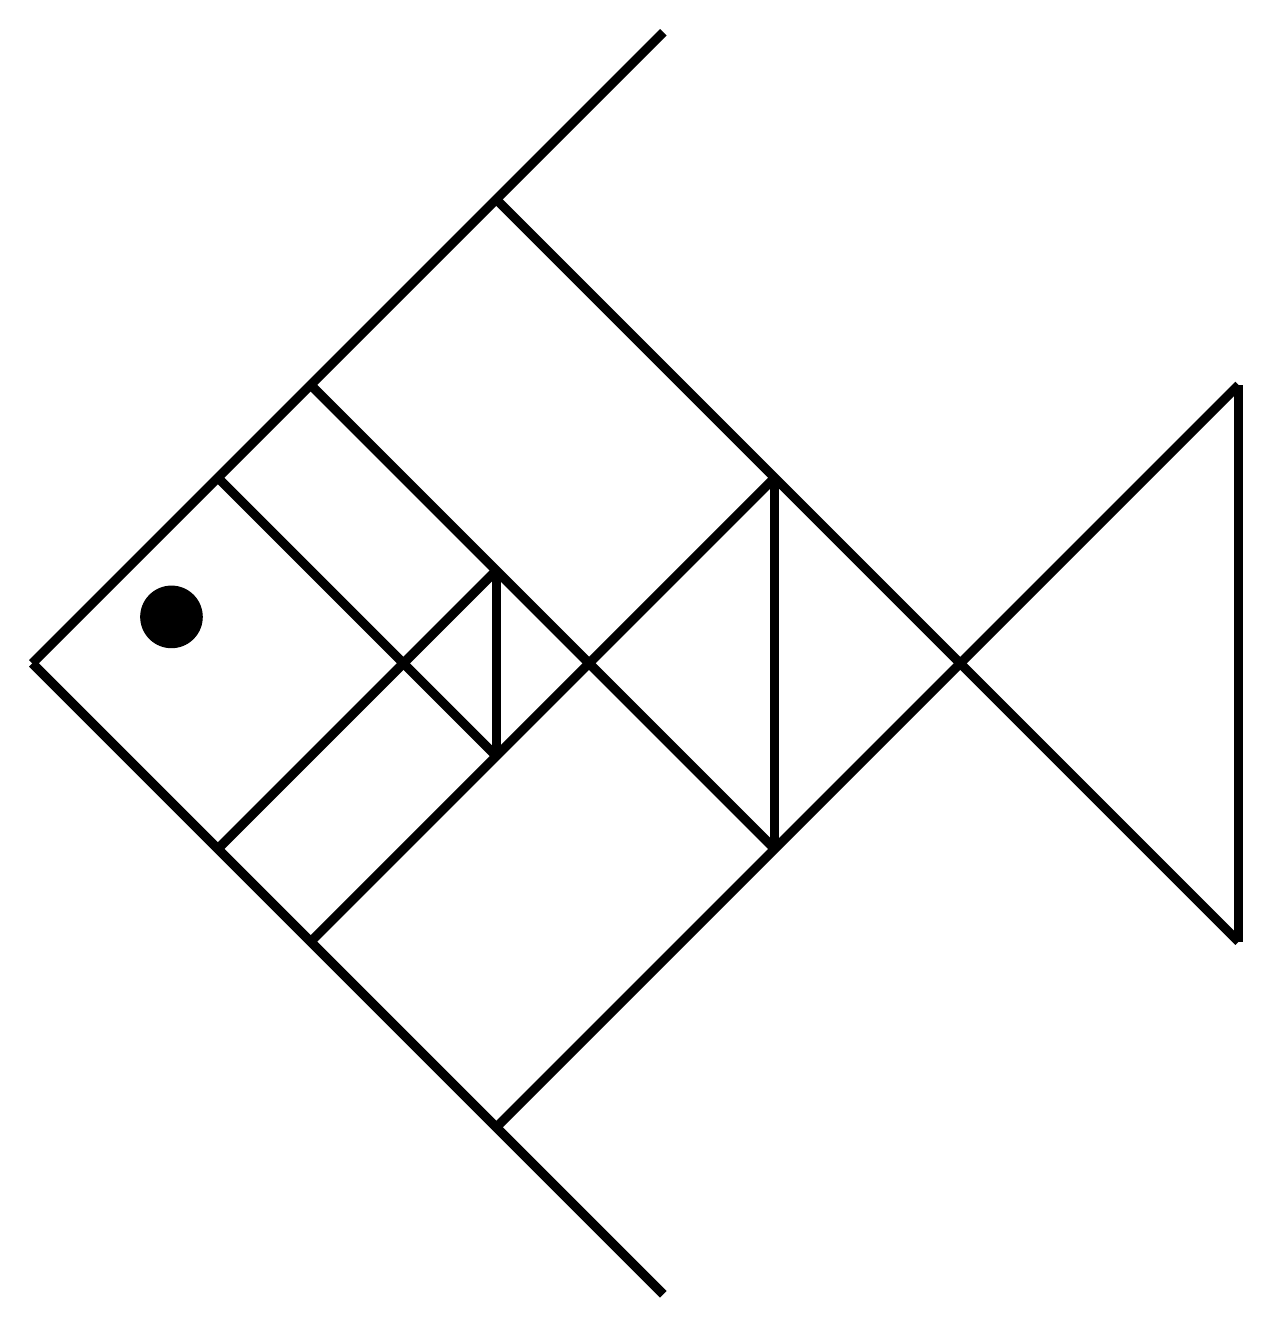
\begin{tikzpicture}[scale=\scal/\pescados,rotate=45,opacity=1]
    \foreach [evaluate={\p=0.5*(\n*(\n-1))+2},evaluate={\c=0.5*((\n*(\n+1))+4}]\n in {1,...,\pescados} {
        \draw [line width=2pt*\scal/\pescados,black] (\p,0)--(\p,-\c);
        \draw [line width=2pt*\scal/\pescados,black] (0,-\p)--(\c,-\p);
        \draw [line width=2pt*\scal/\pescados,black] (\p,-\c)--(\c,-\p);
    }
    \draw[line width=2pt*\scal/\pescados,black](0,0)--(0,{-(0.8*(\pescados*(\pescados-1))+2)});
    \draw[line width=2pt*\scal/\pescados,black](0,0)--({(0.8*(\pescados*(\pescados-1))+2)},0);
    \draw[black,fill=black](1,-0.5) circle (4pt*\scal/\pescados);
\end{tikzpicture}
